% fig_pipeline.tex — AttractorNet overview schematic (vector, standalone)
% Redesigned for print-size legibility: 3 font tiers (>=6.5pt floor, headers >=9pt),
% no truth tables, one simplified thesis inset, 5-gene one-to-one networks, saturated
% agreement marks, fill-redundant node states, generous whitespace.
% Compile: pdflatex fig_pipeline.tex  ->  fig_pipeline.pdf
\documentclass[border=3pt]{standalone}
\usepackage{amssymb}
\usepackage{helvet}
\renewcommand{\familydefault}{\sfdefault}
\usepackage{sansmath}
\sansmath
\usepackage{tikz}
\usetikzlibrary{arrows.meta,positioning,fit,backgrounds,calc}

\definecolor{gnn}{HTML}{2C6FA6}
\definecolor{gnnlt}{HTML}{DCE8F2}
\definecolor{act}{HTML}{3F9C7E}
\definecolor{actlt}{HTML}{D7EAE2}
\definecolor{inh}{HTML}{B5503C}
\definecolor{inhlt}{HTML}{F1DDD7}
\definecolor{mgreen}{HTML}{1C6344}
\definecolor{mred}{HTML}{C0392B}
\definecolor{greyfill}{HTML}{C9CDD2}
\definecolor{greyc}{HTML}{AEB4BA}
\definecolor{greyd}{HTML}{5C6066}
\definecolor{ink}{HTML}{2A2D31}
\definecolor{banner}{HTML}{EDEFF1}

\tikzset{
  % node states (main networks, 5.4mm)
  nN/.style={circle,draw=greyd,line width=0.9pt,fill=greyfill,minimum size=5.4mm,inner sep=0},
  onN/.style={circle,draw=mgreen,line width=0.9pt,fill=act,minimum size=5.4mm,inner sep=0},
  offN/.style={circle,draw=greyd,line width=0.9pt,fill=white,minimum size=5.4mm,inner sep=0},
  % smaller nodes (inset / oracle / model, 4.6mm)
  sN/.style={circle,draw=greyd,line width=0.8pt,fill=greyfill,minimum size=4.6mm,inner sep=0},
  sOn/.style={circle,draw=mgreen,line width=0.8pt,fill=act,minimum size=4.6mm,inner sep=0},
  % signed edges (thick, large heads) for main networks
  Act/.style={draw=act,line width=1.15pt,-{Latex[length=2.5mm,width=2.2mm]},shorten >=8pt,shorten <=8pt},
  Inh/.style={draw=inh,line width=1.25pt,-{Bar[width=3.3mm]},shorten >=8pt,shorten <=8pt},
  % signed edges for smaller graphs
  aAct/.style={draw=act,line width=1.1pt,-{Latex[length=2.3mm,width=2.1mm]},shorten >=6.6pt,shorten <=6.6pt},
  aInh/.style={draw=inh,line width=1.2pt,-{Bar[width=3mm]},shorten >=6.6pt,shorten <=6.6pt},
  % three font tiers
  hdr/.style={font=\fontsize{10}{12}\selectfont\bfseries,text=gnn},
  sub/.style={font=\fontsize{8}{9.5}\selectfont,align=center,text=ink},
  lab/.style={font=\fontsize{8}{9.5}\selectfont,text=ink},
  sm/.style={font=\fontsize{7.5}{9}\selectfont,text=ink},
  smg/.style={font=\fontsize{7.5}{9}\selectfont,text=greyd},
  box/.style={rounded corners=2.5pt,draw,line width=0.8pt,align=center,inner sep=4.5pt,
              font=\fontsize{8}{9.5}\selectfont},
  frame/.style={rounded corners=3pt,draw=greyc,line width=0.6pt},
}

% --- shared 5-gene GRN edge set (local coords); identical in TRANSFER and OUTPUT ---
\newcommand{\grnedges}{%
  \draw[Act] (0.40,0.30)--(0.40,2.95);   % Cln2 -> Clb2
  \draw[Act] (3.25,0.30)--(3.25,2.95);   % Whi5 -> Cdh1
  \draw[Inh] (0.40,2.95)--(1.66,1.72);   % Clb2 -| Sic1 (offset L so the two T-bars separate)
  \draw[Inh] (3.25,2.95)--(1.98,1.72);   % Cdh1 -| Sic1 (offset R)
  \draw[Act] (1.82,1.62)--(0.40,0.30);   % Sic1 -> Cln2
  \draw[Act] (1.82,1.62)--(3.25,0.30);   % Sic1 -> Whi5
}
% agreement mark with white halo: \mk{x}{y}{ok|no}
\newcommand{\mk}[3]{%
  \fill[white] (#1,#2) circle (2.3mm);
  \ifnum\pdfstrcmp{#3}{ok}=0
    \node[font=\fontsize{11.5}{12}\selectfont\bfseries,text=mgreen] at (#1,#2) {\checkmark};
  \else
    \node[font=\fontsize{12}{13}\selectfont\bfseries,text=mred] at (#1,#2) {\sffamily x};
  \fi}

\begin{document}
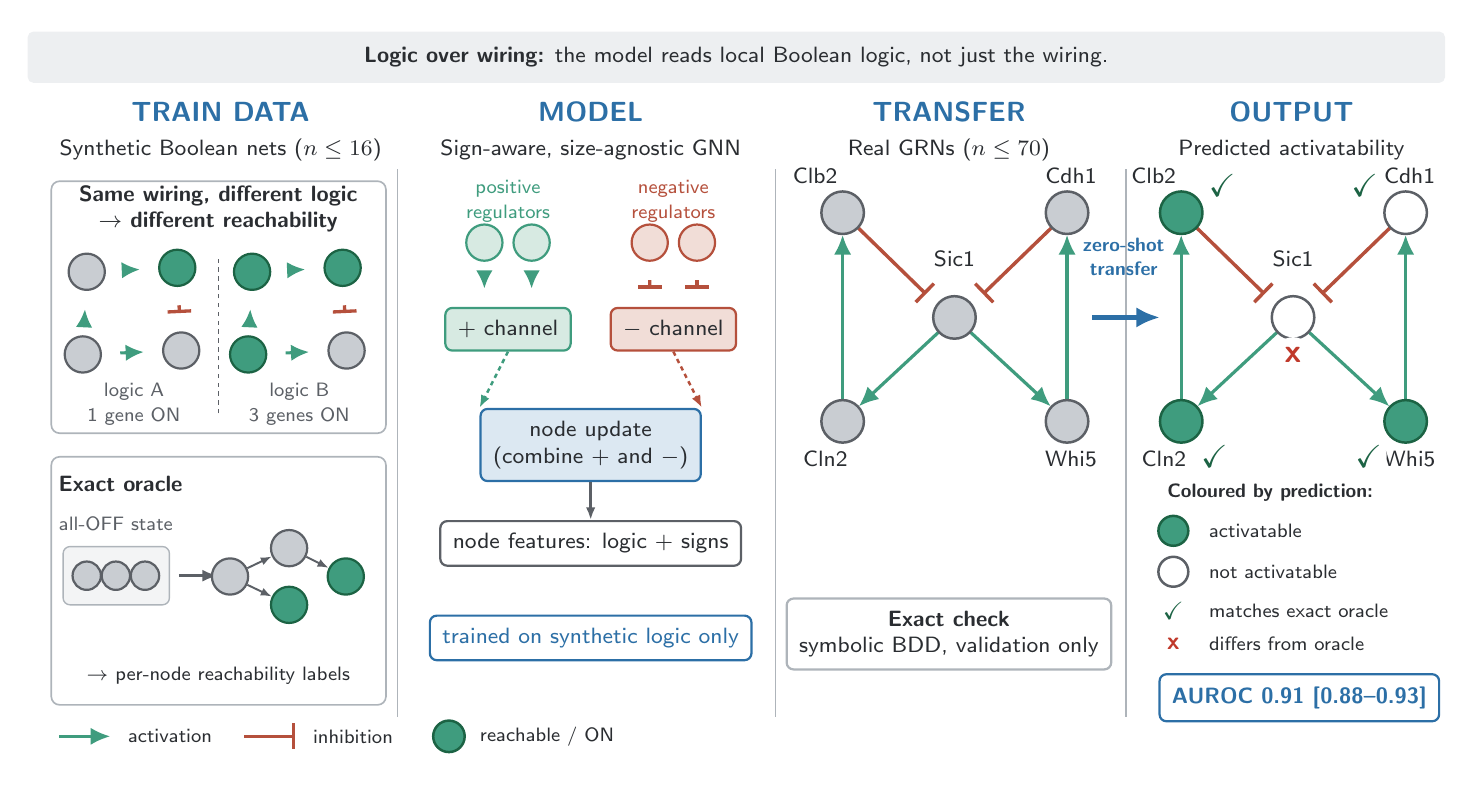
\begin{tikzpicture}
\useasboundingbox (0,-0.1) rectangle (18,9.25);

% ============================ TOP TAGLINE ============================
\fill[banner,rounded corners=2pt] (0,8.55) rectangle (18,9.2);
\node[font=\fontsize{8.5}{10}\selectfont,text=ink] at (9,8.875)
  {\textbf{Logic over wiring:} the model reads local Boolean logic, not just the wiring.};

% ============================ SEPARATORS ============================
\foreach \x in {4.70,9.50,13.95}{\draw[greyc,line width=0.45pt] (\x,0.5)--(\x,7.45);}

% ============================ HEADERS ============================
\node[hdr] at (2.45,8.18){TRAIN DATA};
\node[hdr] at (7.15,8.18){MODEL};
\node[hdr] at (11.7,8.18){TRANSFER};
\node[hdr] at (16.05,8.18){OUTPUT};
\node[sub] at (2.45,7.70){Synthetic Boolean nets ($n\le16$)};
\node[sub] at (7.15,7.70){Sign-aware, size-agnostic GNN};
\node[sub] at (11.7,7.70){Real GRNs ($n\le70$)};
\node[sub] at (16.05,7.70){Predicted activatability};

% ============================ TRAIN: KEY INSET (thesis) ============================
\draw[frame] (0.30,4.10) rectangle (4.55,7.30);
\node[font=\fontsize{8}{9.5}\selectfont\bfseries,text=ink,align=center] at (2.42,6.95)
  {Same wiring, different logic\\$\to$ different reachability};
\draw[greyd,line width=0.5pt,dash pattern=on 1.6pt off 1.6pt] (2.42,4.35)--(2.42,6.35);
% left network: logic A -> little reachable
\begin{scope}[shift={(0.45,4.95)}]
  \node[sN] (LA) at (0.30,1.20){}; \node[sOn] (LB) at (1.45,1.25){};
  \node[sN] (LC) at (1.50,0.20){}; \node[sN] (LD) at (0.25,0.15){};
  \draw[aAct] (LA)--(LB); \draw[aInh] (LB)--(LC); \draw[aAct] (LD)--(LC); \draw[aAct] (LD)--(LA);
\end{scope}
\node[sm,text=greyd,align=center] at (1.35,4.47){logic A\\1 gene ON};
% right network: SAME wiring, logic B -> more reachable
\begin{scope}[shift={(2.55,4.95)}]
  \node[sOn] (RA) at (0.30,1.20){}; \node[sOn] (RB) at (1.45,1.25){};
  \node[sN] (RC) at (1.50,0.20){}; \node[sOn] (RD) at (0.25,0.15){};
  \draw[aAct] (RA)--(RB); \draw[aInh] (RB)--(RC); \draw[aAct] (RD)--(RC); \draw[aAct] (RD)--(RA);
\end{scope}
\node[sm,text=greyd,align=center] at (3.45,4.47){logic B\\3 genes ON};

% ============================ TRAIN: EXACT ORACLE ============================
\draw[frame] (0.30,0.65) rectangle (4.55,3.80);
\node[lab] at (1.18,3.46){\textbf{Exact oracle}};
% all-OFF state: the genes (all grey) grouped as ONE start state
\draw[rounded corners=2.5pt,draw=greyc,line width=0.5pt,fill=greyc!15] (0.45,1.92) rectangle (1.80,2.66);
\node[sm,text=greyd] at (1.12,2.95){all-OFF state};
\node[sN,minimum size=3.6mm] at (0.75,2.29){}; \node[sN,minimum size=3.6mm] at (1.12,2.29){};
\node[sN,minimum size=3.6mm] at (1.49,2.29){};
\draw[-{Latex[length=2mm]},line width=1pt,greyd] (1.92,2.29)--(2.42,2.29);
% reachability tree (green = states a gene becomes reachable)
\begin{scope}[shift={(2.52,1.66)}]
  \node[sN] (t0) at (0.05,0.62){}; \node[sN] (t1) at (0.80,0.98){}; \node[sOn] (t2) at (0.80,0.26){};
  \node[sOn] (t3) at (1.52,0.62){};
  \draw[-{Latex[length=1.4mm]},line width=0.7pt,greyd] (t0)--(t1);
  \draw[-{Latex[length=1.4mm]},line width=0.7pt,greyd] (t0)--(t2);
  \draw[-{Latex[length=1.4mm]},line width=0.7pt,greyd] (t1)--(t3);
\end{scope}
\node[sm] at (2.42,1.02){$\to$ per-node reachability labels};

% ============================ MODEL ============================
% regulators sit ABOVE their channel box so the signed arrows have vertical room
\node[sm,text=act,align=center] at (6.10,7.04){positive\\regulators};
\node[sm,text=inh,align=center] at (8.20,7.04){negative\\regulators};
\node[sN,fill=actlt,draw=act] (p1) at (5.80,6.52){}; \node[sN,fill=actlt,draw=act] (p2) at (6.40,6.52){};
\node[sN,fill=inhlt,draw=inh] (q1) at (7.90,6.52){}; \node[sN,fill=inhlt,draw=inh] (q2) at (8.50,6.52){};
\node[box,draw=act,fill=actlt,text=ink] (pch) at (6.10,5.42){$+$ channel};
\node[box,draw=inh,fill=inhlt,text=ink] (qch) at (8.20,5.42){$-$ channel};
\draw[aAct] (p1)--([xshift=-3mm]pch.north); \draw[aAct] (p2)--([xshift=3mm]pch.north);
\draw[aInh] (q1)--([xshift=-3mm]qch.north); \draw[aInh] (q2)--([xshift=3mm]qch.north);
\node[box,draw=gnn,fill=gnnlt,text=ink] (upd) at (7.15,3.95){node update\\(combine $+$ and $-$)};
\draw[draw=act,line width=0.9pt,dash pattern=on 1.6pt off 1.4pt,-{Latex[length=1.6mm]}] (pch.south)--(upd.north west);
\draw[draw=inh,line width=0.9pt,dash pattern=on 1.6pt off 1.4pt,-{Latex[length=1.6mm]}] (qch.south)--(upd.north east);
\node[box,draw=greyd,fill=white,text=ink] (feat) at (7.15,2.70){node features: logic $+$ signs};
\draw[-{Latex[length=1.6mm]},line width=0.9pt,greyd] (upd.south)--(feat.north);
\node[box,draw=gnn,fill=white,text=gnn,minimum width=4.0cm] (badge) at (7.15,1.50)
  {trained on synthetic logic only};

% ============================ TRANSFER ============================
\begin{scope}[shift={(9.95,3.95)}]
  \grnedges
  \node[nN] at (0.40,2.95){}; \node[nN] at (3.25,2.95){}; \node[nN] at (1.82,1.62){};
  \node[nN] at (0.40,0.30){}; \node[nN] at (3.25,0.30){};
  \node[lab] at (0.05,3.42){Clb2}; \node[lab] at (3.30,3.42){Cdh1};
  \node[lab,fill=white,inner sep=1pt] at (1.82,2.36){Sic1}; \node[lab] at (0.18,-0.18){Cln2}; \node[lab] at (3.30,-0.18){Whi5};
\end{scope}
% zero-shot arrow
\node[font=\fontsize{7}{8.5}\selectfont\bfseries,text=gnn,align=center] at (13.92,6.34){zero-shot\\transfer};
\draw[-{Latex[length=3mm,width=2.6mm]},line width=2pt,gnn] (13.52,5.57)--(14.38,5.57);
% exact check chip
\node[box,draw=greyc,fill=white,text=ink,align=center] at (11.7,1.55)
  {\textbf{Exact check}\\symbolic BDD, validation only};

% ============================ OUTPUT ============================
\begin{scope}[shift={(14.25,3.95)}]
  \grnedges
  \node[onN] at (0.40,2.95){}; \node[offN] at (3.25,2.95){}; \node[offN] at (1.82,1.62){};
  \node[onN] at (0.40,0.30){}; \node[onN] at (3.25,0.30){};
  \node[lab] at (0.05,3.42){Clb2}; \node[lab] at (3.30,3.42){Cdh1};
  \node[lab,fill=white,inner sep=1pt] at (1.82,2.36){Sic1}; \node[lab] at (0.18,-0.18){Cln2}; \node[lab] at (3.30,-0.18){Whi5};
  \mk{0.92}{3.30}{ok}   % Clb2 matches
  \mk{2.73}{3.30}{ok}   % Cdh1 matches
  \mk{1.82}{1.14}{no}   % Sic1 differs (anchored just below its node)
  \mk{0.82}{-0.14}{ok}  % Cln2 matches (beside its label, clear of the green node)
  \mk{2.78}{-0.14}{ok}  % Whi5 matches (beside its label, clear of the green node)
\end{scope}
% legend
\node[font=\fontsize{7}{8.5}\selectfont\bfseries,text=ink,anchor=west] at (14.35,3.34){Coloured by prediction:};
\node[onN,minimum size=3.8mm] at (14.55,2.86){};
\node[sm,anchor=west] at (14.88,2.86){activatable};
\node[offN,minimum size=3.8mm] at (14.55,2.34){};
\node[sm,anchor=west] at (14.88,2.34){not activatable};
\node[font=\fontsize{9}{10}\selectfont\bfseries,text=mgreen] at (14.55,1.84){\checkmark};
\node[sm,anchor=west] at (14.88,1.84){matches exact oracle};
\node[font=\fontsize{9.5}{10}\selectfont\bfseries,text=mred] at (14.55,1.42){\sffamily x};
\node[sm,anchor=west] at (14.88,1.42){differs from oracle};
% AUROC
\node[box,draw=gnn,fill=white,text=gnn,font=\fontsize{8}{9.5}\selectfont\bfseries,align=center,minimum width=2.9cm]
  at (16.15,0.74){AUROC 0.91 [0.88--0.93]};

% ============================ BOTTOM SIGN LEGEND ============================
\draw[Act,shorten >=0pt,shorten <=0pt] (0.40,0.25)--(1.05,0.25);
\node[sm,anchor=west] at (1.15,0.25){activation};
\draw[Inh,shorten >=0pt,shorten <=0pt] (2.75,0.25)--(3.40,0.25);
\node[sm,anchor=west] at (3.50,0.25){inhibition};
\node[onN,minimum size=4mm] at (5.35,0.25){};
\node[sm,anchor=west] at (5.62,0.25){reachable / ON};

\end{tikzpicture}
\end{document}
